\section{Оружие}
Порой от выбора оружия зависит жизнь или смерть героя. Впрочем, иногда оружие — всего лишь деталь социального статуса или стильное дополнение к костюму.
\paragraph{Бонус к Повреждениям (БПв):} опытный боец опасен сам по себе. Однако большинство воинов предпочитают иметь при себе оружие. Оружие дает Бонус к Повреждениям, который прибавляется к Доблести и Меткости. Бонус постоянен и зависит от выбранного оружия. Чем он больше, тем смертоноснее оружие в умелых (или даже не очень умелых) руках.
\paragraph{Дистанция поражения:} в бою герой может атаковать противника в одном метре от себя (в соседней клетке, если используется масштабная карта). У дальнобойного оружия есть две дистанции — Ближняя, на которой оружие наиболее опасно, и Дальняя, предельная дистанция, на которой возможно поражение цели. Как правило, БПв на Дальней дистанции ниже, чем на Ближней, иногда значительно.
\paragraph{Бонус/Штраф размера и дистанция поражения:} чем больше существо, тем проще ему атаковать цели, не стоящие к нему вплотную. Совершая вооруженные атаки в ближнем бою, существо прибавляет свой БШР к дистанции поражения, а оружие получает свойство «Длинное». Например, двуручный меч в руках Большого огра будет иметь дистанцию поражения 2. БШР не может понизить дистанцию поражения до 0, то есть даже кинжал в руках Крошечной феи будет иметь дистанцию поражения 1.
\paragraph{Требуемая Сила (тСл):} для успешного использования оружия нужно быть сильным. Хилый герой не натянет лук и не рубанет двуручным топором как следует. 
\newline
Если значение силы героя меньше Требуемой Силы оружия, то все атаки им он совершает с Помехой. Герой, не имеющий достаточной Силы, не может сражаться Громоздким оружием вообще. Конечно, он вполне способен размахивать им и даже выглядеть при этом угрожающе, но нанести ущерб может разве что случайно (например, если герой Неуклюжий).
\paragraph{Единицы Здоровья (ЕЗ) оружия = |1/2 минСл|.} Например, двуручный меч имеет минСл 12, значит у него 6 ЕЗ. Если у оружия несколько параметров минСл, используйте наибольший для определения ЕЗ.
\paragraph{Прочность (Прч) оружия = |1/2 ЕЗ оружия|.} Оружие имеет показатель Прочности. Прочность вычитается из Пв, которые получает предмет.
\paragraph{Критический Удар(КУ):} минимальное число на кубике, при выпадении которого применяются критические эффекты на цель. Критические эфекты налагаются только в дополнение к эфектам попадания по цели. Например, если герой наносит удар с Доблестью +2 и КУ 17 против цели с ЗЩ 25 и на кубике выпало 18, то это все еще промах и эфект КУ не применяется.
\paragraph{Халтура, работа мастера и шедевр:} дешевое, кое-как изготовленное оружие (вроде того, которым сражаются ратные холопы) имеет 1/2 ЕЗ, 1/2 Прч и -1 к БПв. Дешевое оружие получает Осечку 5 и ломается при Критическом провале Дб или Мт. Понизьте СП на 5 (минимум 1 СП).
\newline Оружие, изготовленное мастером, имеет +1 к БПв. Параметр минСл уменьшается на 1 (это не влияет на ЕЗ предмета). Повысьте СП на 5.
\newline
Шедевр представляет собой безупречный экземпляр мастерской работы и получает все преимущества работы мастера. Увеличьте ЕЗ предмета в 1.5 раза. Шанс КУ такого оружия возрастает на 1, то есть меч будет наносить КУ на 18, 19 и 20, а топор на 19 и 20. Повысьте СП на 10.
\paragraph{Владение различными видами оружия:} видов оружия великое множество. Редкий воин обладает талантом (и временем для тренировок), позволяющим освоить их все. К тому же во многом это вопрос привычки — порой даже два вроде бы похожих меча ощущаются по-разному, если одним из них воин фехтовал полжизни, а другой лишь вчера взял в руку.
\newline
В начале игры герой должен выбрать число видов оружия, которыми он умеет пользоваться, равное \textbf{|3 + МИн|}. Этот набор сам по себе немало расскажет о герое — откуда он, почему научился владеть именно этими видами оружия и именно в таком сочетании. Не упускайте шанс добавить образу глубины! При использовании любого оружия, которого нет в перечне, герой получает Помеху при проверке Доблести и Меткости. Чтобы научиться владеть оружием в полной мере и избавиться от Помехи, герой должен потратить 2 Очка опыта. Это может отображать долгие упражнения, которыми герой изнурял себя, пока друзья посиживали в трактирах, либо понимание общих принципов действия оружия или даже внезапное озарение, если это не идет в разрез с настроением вашей истории.
\newline
Не забывайте, что если герой не распределил Очки опыта во Владение оружием, Рукопашный бой или Стрельбу, то соответствующие проверки Доблести и Меткости совершаются им с Помехой. То есть если в руках такого героя оказалось незнакомое оружие, он получает 2 Помехи!
\paragraph{Импровизированное оружие:} может обладать любыми свойствами и типом Пв. Например, вилы Длинные и Колющие, а оглобля Громоздкая и Дробящая. Как правило, большинство Импровизированного оружия напоминает боевое. Из разбитой пивной кружки получится превосходный кастет, а из дамской сумочки — цеп. Обычно БПв, Прч и ЕЗ импровизированного оружия
ниже, чем у его боевого аналога.
\paragraph{Удары плашмя:} абсолютное большинство видов рубящего и колющего оружия можно использовать для ударов плашмя. Это редко имеет смысл в бою насмерть, но неплохо работает в тех случаях, когда противник хорошо защищен от колющих или режущих атак, а также если требуется захватить его относительно невредимым. Удары плашмя наносятся с Помехой и имеют Дробящие Пв. Дальнобойные атаки также могут использовать это правило — стрелок пускает стрелу или пулю вскользь. Удары плашмя могут (но не обязаны) следовать правилам Несмертельных Пв.
\paragraph{Несмертельные Повреждения:} иногда героям требуется захватить противника живьем. Для этих ситуаций идеально подходит оружие, наносящее Дробящие Пв. При атаке таким оружием герой может нанести Несмертельные Пв, равные |1 + ММд/Врачевание (Мд)|. Игрок должен объявить, что герой наносит Несмертельные Пв.
Несмертельные Пв отнимаются от общего числа ЕЗ жертвы и могут привести к Опасной ране и прочим эффектам. Сломанные и отрубленные благодаря Несмертельным Пв конечности считаются вывихнутыми, если наносящий Пв герой того пожелает. Все КУ, вызыванные Несмертельными Пв, приводят к Оглушению. Если атака героя приводит к смерти жертвы, он может объявить, что жертва потеряла сознание и осталась жива. Потерянные от Несмертельных Пв ЕЗ восстанавливаются со скоростью 1 ЕЗ за 10 минут отдыха (даже если отдых — это лежание на холодной земле со связанными руками и ногами).
\newline
Когда при ударе жертва получает и Несмертельные, и обычные Пв, это может привести к Смерти или Перелому, если Мудрость или Врачевание наносящего удар героя недостаточно высоки!
\paragraph{Оружие для больших и маленьких существ}
В таблицах представлено оружие, изготовленное для существ Среднего размера. Для существ иного размера оружие должно изготовляться под их размер. Понизьте БПв оружия на 1 за каждую категорию размера существа меньше Среднего и повысьте на 1 за каждую категорию размера больше Среднего. Также повысьте СП оружия на 2 за каждую категорию размера существа больше Среднего — большое оружие стоит дороже! Стоимость оружия для маленьких существ не меняется — меньшая стоимость материалов компенсируется сложностью работы. Увеличение СП за размер складывается с изменением СП за Халтуру, Работу мастера или Шедевр.
\newline
Таким образом, короткий меч с БПв +1 будет иметь БПв +0, если выкован для Маленького карлика. Изготовленный для Большого великана, короткий меч будет иметь БПв +2 и СП 8 вместо 6.
Маленькие и Крошечные существа могут применять оружие большего размера как двуручное без увеличения минСл, если только оно не Громоздкое. Например, Маленький карлика может использовать обычный меч с БПв +2 как Двуручное оружие.
Конечно, карлика предпочел бы двуручный меч, выкованный специально для него (такой меч имел бы БПв +3), но бывают ситуации, когда выбирать не приходится! Или, например, он мог бы использовать короткий меч из таблицы как обычный меч. При этом короткий меч лишится свойства «Легкое», ведь для карлика он совсем не легкий! Зато пара кинжалов послужила бы карлика не хуже, чем пара коротких мечей — человеку.
\newline
Высокая Сила позволяет герою частично обойти эти ограничения и сохранить БПв и свойства оружия. Повысьте минСл оружия на 3 для Маленьких существ и на 6 — для Крошечных. Понизьте минСл оружия на 3 для Больших существ, на 6 — для Огромных и на 9 — для Громадных. Если в результате понижения минСл она достигает 3/4 от изначальной, значит, существо может использовать оружие как одноручное. Если в результате понижения минСл она достигает 1/2 от изначальной, значит, существо может использовать оружие как одноручное, и оружие получает свойство «Легкое». Если в результате понижения минСл оружия получается 0 или меньше, существо не может эффективно использовать оружие в бою — оно больше подойдет ему в качестве зубочистки!
\paragraph{ЕЗ оружия для больших и маленьких существ:} повысьте ЕЗ оружия в 1.5 раза за каждую категорию размера больше Среднего и понизьте в 1.5 раза за каждую категорию размера меньше Среднего. Например, двуручный меч для Среднего человека имеет 6 ЕЗ и Прч 3. Двуручный меч для Маленького карлика будет иметь 4 ЕЗ и Прч 2, а двуручный меч для Большого великана — 9 ЕЗ и Прч 4!
\subsection{Cвойства оружия}
\paragraph{Бронебойное:} оружие ополовинивает Бонус доспеха и щита цели. Обратите внимание, что это свойство не влияет на Прочность цели.
\paragraph{Боеприпасы:} некоторые виды оружия нуждаются в боеприпасах. Без них оно  — всего лишь безделушка(хотя если это что-то тяжелое, им можно орудовать, как импровизированным оружием ближнего боя). СП 10 зарядов для любого вида оружия и 1 заряда для Противотанкового оружия равна \textbf{|СП оружия — 10|}. Стоимость 1 заряда для любого оружия, кроме Противотанкового равна \textbf{|СП оружия — 15|} (минимум 1).
\paragraph{Возврат Х:} при выпадении Х или большего числа во время проверки Мт оружие не только наносит Пв, но и возвращается в руку к владельцу.
\paragraph{Громоздкое:} используется с Помехой в тесных помещениях и густых зарослях. Если оружие одновременно и Громоздкое, и Длинное, герой получает 2 Помехи. Герой не может использовать Громоздкое оружие лежа для атак в ближнем бою.
\paragraph{Двуручное:} требует 2 рук для использования.
\paragraph{Дистанция X/Y:} Оружие с этим свойством является дальнобойным и не предназначено для совершения атак в ближнем бою. \textbf{X} - Ближняя Дистанция оружия, \textbf{Y} - Дальняя Дистанция оружия. В графе БПв для этго оружия через черту написан урон для Ближней и Дальней дистанции соответственно.
\paragraph{Длинное:} позволяет атаковать врага в 2 метрах от героя. Цели, находящиеся ближе, герой атакует с Помехой. Длинное оружие используется с Помехой в тесных помещениях, густых зарослях и других подобных условиях.
\paragraph{Кавалерийское:} удвойте успешно нанесенные Пв, если геройверхом и применяет Атаку с разбега.
\paragraph{Кастет:} позволяет использовать как Навык Рукопашного боя, так и Навык Владения оружием в формуле Дб.
\paragraph{Класс повреждений Х(КП Х):} Добавляет значение Х к Размеру оружия для определения условий Подавляющего превосходства, не меняя размер оружия для определения других его свойств.

\paragraph{Кувалда:} если нанесенные Пв превышают МСл атакованного существа, оно падает. 
\newline
Маленькие существа падают, если нанесенные Пв превышают 1/2 их МСл, Крошечные — падают, если нанесенные Пв превышают 1/4 их МСл.
\newline
Большие существа падают, если нанесенные Пв превышают их МСл более чем в 2 раза, Огромные — если нанесенные Пв превышают их МСл более чем в 3 раза, Громадные — если нанесенные Пв превышают их МСл более чем в 4 раза.
\newline
Если оружие ближнего боя с этим свойством используется в одной руке, увеличьте необходимые для падения Пв в 2 раза. То есть для того, чтобы сбить с ног существо Среднего размера, понадобится превысить его МСл более чем в 2 раза.
\paragraph{Легкое:} позволяет совершать серии молниеносных выпадов и эффективно атаковать с оружием в каждой руке.
\paragraph{Тип оружия:} Любое дальнобойное оружие нуждается в боеприпасах. Но благодаря унификации герою не нужно носить разные боеприпасы для \textit{каждой} еденицы оружия, которая есть у него в арсенале. Стоимость и свойства боеприпасов описаны в следующем разделе. Тип оружия определяет тип боеприпасов, который использует это оружие:
\begin{center}
\begin{tabular}{|c|p{3cm}|p{10cm}|}
\hline
Тип & Описание & Описание боеприпасов\\ \hline
Р & револьверы и крупнокалиберные пистолеты & медленные пули, которые обычно легко купить\\ \hline
В & винтовки & быстрые пули с хорошей пробивающей способностью\\ \hline
Д & дробовики & дробь и картечь. Реже - пули\\ \hline
О & пулеметы и крупнокалиберные орудия & действительно большие калибры. Размеры настолько высоки, что в них можно поместить взрывчатку\\ \hline
Г & гранатометы и ракетные установки & Унифицированные гранаты и ракеты. Поражающий эффект зависит от начинки\\ \hline
Э & энергетическое оружие & Батареи всех пород и мастей. Если у оружия класса Э нет свойства Потребления, оно тратит 1 Заряд за выстрел.\\ \hline
Б\textsuperscript{ф} & кинетические ускорители & Металические болты с сверхтвердым сердечником. Дешевы в изготовлении, но если их хорошенько разогнать, становятся крайне смертоносны.\\ \hline
М & метательное & Оружие использует метательный боеприпас и приводится в действие силой стрелка. \\ \hline
У & уникальный боеприпас & Оружие использует не стандартизированный боеприпас, который подойдет только для него. СП 10 зарядов для такого вида оружия равна \textbf{|СП оружия — 10|}. Стоимость 1 заряда для этого оружия равна \textbf{|СП оружия — 12|} (минимум 1). \\ \hline
\end{tabular}
\end{center}
\paragraph{Магазин/Скорострельность(МСк) Х/Y:} дальнобойное оружие с этим свойством способно выпускать множество снарядов сразу или один за другим и не требовать Перезарядки сразу после первого выстрела. \textbf{X} количество выстрелов, которое может сделать оружие без Перезарядки, а \textbf{Y} — число выстрелов, которое герой может произвести за время своего Действия. Скорострельное оружие может использоваться двумя способами — для поражения одной цели или нескольких. При использовании скорострельного оружия герой может одновременно поразить число целей, не превышающее его \textbf{|ММд+1|} (минимум 2 цели).
\newline
Если Скорострельное оружие используется против одной цели, повысьте БПв оружия на 1 за каждый снаряд после первого, выпущенный по ней. Например, скорострельный арбалет имеет БПв +1 и Скорострельность 3. Если герой трижды стреляет из скорострельного арбалета в одну цель, БПв скорострельного арбалета возрастает до +3 (то есть на 2).
Герой не может совершать Быструю атаку скорострельным оружием, но может использовать место этого Беглый огонь. В разделе Маневры есть полное описание этого маневра.
\begin{tcolorbox}
Если у оружие есть свойство Магазин или Потребление, то это значит, что у оружия есть свойство Перезарядка, даже если это явно не указано. Оружие с МСк надо Перезаряжать, когда закончатся заряды в магазине, а оружие с Потреблением - когда опустошена Энергоячейка.
\end{tcolorbox}
\paragraph{Тип/Магазин/Скорострельность(ТМС):} объедененный столбец, в котором через черту отражены класс оружия, размер магазина и его скорострельность.
\paragraph{Метательное:} может быть использовано и в ближнем и в дальнем бою. При метании оружие обычно падает в область, в которой находилась цель. Оно может быть поднято и использовано повторно. При Дистанционной атаке Метательным оружием герой добавляет свой МСл к БПв оружия. У метательного оружия \textbf{нет} свойства Перезарядка - количество выстрелов в раунд ограничена только Скорострельностью оружия. Если герой держит в каждой руке два одинаковых Метательных оружия, он может метнуть оба в рамках маневра Беглый огонь или Атака, повысив скорострельность оружия на 1, но получив при этом Помеху на этом маневр и дополнительно вторую Помеху, если оружие Громоздкое. Если у героя есть трюк Амбидекстер, он получает на одну Помеху меньше при совершении этого маневра. В таблицах свойство Метательное указано в столбце ТМС как тип оружия.
\begin{tcolorbox}
Используя метательное оружие с дополнительным свойством \textbf{Снаряды} герой не метает оружие целиком, а использует подготовленные для него снаряды. Им нельзя производить атаку в Ближнего боя, однако стоимость выстрела гораздо ниже, когда во врага летит только часть оружия. СП 10 зарядов для такого вида оружия равна \textbf{|СП оружия — 10|}. Стоимость 1 заряда для этого оружия равна \textbf{|СП оружия — 12|} (минимум 1).
\end{tcolorbox}
\paragraph{Огнемет:} при атаке огнемет поражает все объекты, находящиеся на линии между стрелком и целью атаки. Совершите только одну проверку Меткости и определите повреждения для всех пораженных объектов, исходя из нее. В случае выпадения КУ его эффекты применяются ко всем объектам, пораженным огнеметом.
\paragraph{Отдача:} герой должен отказаться от Перемещения, если желает выпустить из оружия с этим свойством 5 или больше зарядов.
\paragraph{Перезарядка:} для перезарядки оружия с этим свойством герой должен отказаться от Действия или Перемещения. Оружие не может использоваться при Быстрой атаке. Арбалеты и пороховое оружие требуют 2 свободных рук при перезарядке.
\paragraph{Потайное:} герой получает Преимущество на проверки Скрытности и Ловкости рук при попытках спрятать оружие.
\paragraph{Потребление Х:} Оружие с этим свойством вместо боеприпасов использует энергию и тратит Х Зарядов за 1 выстрел или удар.
%\paragraph{Противотанковое:} оружие предназначено для поражения тяжелобронированных целей. У остальных не так уж много шансов пережить попадание из него. При произведении выстрела из противотанкового оружия, \troubleControl Меткости против ЗЩ цели.
%\trouble
%{В яблочко}%no sweat name
%{Цель зацепило снарядом. Она теряет все свои ЕЗ.}%no sweat description
%{Прямое попадание}%tough day name
%{Цель слегка задело. Она теряет 1/2 своих ЕЗ.}%tough day description
%{Попадание}%we have trouble name
%{Цель задело осколками или взрывом. Она теряет 1/4 своих ЕЗ.}%we have trouble description
%{Промах}%fiasco name
%{Цель обдало грязью, травой, мелкими камушками (и, возможно, останками тех, кому повезло меньше), но в остальном она невредима}%fiasco description
\paragraph{Пулемет:} оружие не приспособлено для одиночных выстрелов. Если герой использует оружие для поражения нескольких целей, то должен выпустить минимум 3 пули в каждую.
\paragraph{Снайперское:} при стрельбе на дальнюю дистанцию оружие игнорирует штрафы Зон поражения, если герой проводит Прицеливаясь хотя бы один полный Круг. При стрельбе на ближней дистанции герой получает Помеху.
\paragraph{Сошки(с):} оружие оснащено сошками для стрельбы с упора. Если носитель имеет возможность установить сошки на какую-либо поверхность, используйте значение Минимальной силы с пометкой (с), в противном случае используйте значение после черты. Если у оружия нет значения Минимальной силы без символа (с), значит, стрельба с рук невозможна.
\paragraph{Тип Повреждений:}
в зависимости от типа, повреждения могут иметь разные эффекты КУ и могут быть увеличены или уменьшены в зависимости от того, какие есть сопротивления или уязвимости у цели. Атаки имеют один из следующих типов Повреждений:
\newline
\textbf{(Д)}робящие, \textbf{(Е)}дкие, \textbf{(К)}олющие, \textbf{(Л)}едяные, \textbf{(О)}гненные, \textbf{(П)}роникающие, \textbf{(Р)}убящие, \textbf{(Э)}лектрические, \textbf{(Я)}довитые.
\newline
Если тип повреждений отмечен *, то он зависит от заряженных в оружие боеприпасов. См. раздел боеприпасов для определения типа повреждений.
\newline
Если оружие имеет несколько типов повреждений через черту(К/Р или Р/Д), герой может выбирать, какой тип повреждений наносить при атаке. Если типы повреждений перечислены слитно(ОЭ или РЯ), то оружие наносит одновременно несколько типов повреждений. Подробнее об этом написано в главе Боевые Столкновения.
\paragraph{Удавка:} этим свойством обладает любое оружие, достаточно гибкое, чтобы захлестнуть конечности противника. Для применения свойства необходимо две руки. Оружие может использоваться для Захватов. Удвойте Пв, успешно нанесенные Удавкой в шею. Существа, чьи ЕЗ опустились до 0 в результате Пв, нанесенных Удавкой в шею, теряют сознание, а не умирают, если атакующий того пожелает. Существа, у которых БДЗщ (но не БЩЗщ) составляет 6 или больше, не могут быть атакованы Удавкой в шею — она надежно защищена.
\paragraph{Универсальное:} может использоваться в 1 или 2 руках. Смена хвата является Быстрым действием. В БПв и тСл указаны для одной и двух рук через черту.
\paragraph{Упредительный удар:} если противник входит в зону поражения оружия, герой может потратить Быстрое действие и провести внеочередную атаку по нападающему или его скакуну. Выход из зоны действия оружия и передвижение в ней не провоцируют Упредительный удар.
\paragraph{Фехтовальное:} герой может заменить МСл на ММд при подсчете Дб.
\paragraph{Хрупкое:} из-за особенностей конструкции оружие уязвимо к самым незначительным повреждениям и не предназначено для парирования и блокирования. Ополовиньте ЕЗ оружия(минимум 1 ХП).
\paragraph{Цеп:} игнорирует БЩЗщ, хотя может заявлять щит как область поражения.
\paragraph{Символ «*»} обозначает качества оружия, не указанные в таблице, не входящие в унифицированный перечень Свойств и перечисленные в описательном блоке. \textbf{Символ «Ф»} обозначает оружие, уместное лишь в фантастическом антураже.
\subsection{Боеприпасы дальнобойного оружия}

\tbd


\subsection{Оружие ближнего боя}
\genAndGet{weapons}{meleeWeapons}

\subsection{Вспомогательное и импровизированное оружие}
Все, что не является оружием, можно использовать как оружие. Но некоторые вещи просто напрашиваются на то, чтобы ими кого-нибудь ударили, порезали или проткнули.
\genAndGet{weapons}{supplimentalWeapons}

\subsection{Дальнобойное оружие прошлого}
\genAndGet{weapons}{elderWeapons}

\subsection{Современное дальнобойное оружие}
\genAndGet{weapons}{modernWeapons}

\subsection{Дальнобойное оружие будущего}
\genAndGet{weapons}{futureWeapons}

\subsection{Гранаты и взрывы}
\paragraph{}
В историях всегда найдется место бутылкам с горючей смесью, емкостями с едкими летучими веществами и старым добрым гранатам. И это, и многое другое можно метнуть во врага. А потом наблюдать с безопасного расстояния, как он мечется в бессильных попытках погасить пламя, истекает кровью, изрешеченный осколками… или как бутыль предательски падает в траву, а отсыревший запал гаснет.
\paragraph{}
Гранаты — Метательное оружие с БПв = \textbf{|МСл — 2|} на Ближней и \textbf{|МСл — 4|} на Дальней дистанции. Непосредственно удар гранаты имеет Дробящие Пв и наносит КУ при выпадении 20. Используйте Мт, чтобы определить, поразил ли герой цель. Не забывайте, что гранаты можно метать в землю, поражая Зщ 10, если только герой не собирается нанести Повреждения самим броском!
\newline
Все бомбы и гранаты считаются одним видом оружия.
\paragraph{}
В случае промаха граната все равно взорвется (если только не выпала Осечка). Граната отклоняется на Х метров, где Х равен промаху героя по Зщ цели — ловкий противник может успеть отбросить гранату, а бронированный — отбить щитом или латным рукавом! Определите направление, в котором отклонилась граната, при помощи броска К20. В этом случае граната может пролететь большее расстояние, чем максимальная дистанция броска!
\begin{center}
\begin{tabular}{ |p{2.7cm}|p{12cm}| }
\hline
\textbf{К20} & \textbf{Направление}
\\ \hline
1-5 & Граната перелетела за цель
\\ \hline
6-10 & Граната отклонилась вправо от цели
\\ \hline
11-15 & Граната недолетела до цели
\\ \hline
16-20 & Граната отклонилась влево от цели
\\ \hline
\end{tabular}
\end{center}
\begin{tcolorbox}
Если нужно больше детализации по направлению, можно использовать принцип дартс: область вокруг цели делится на 20 равных секторов и каждому из них сопоставляется число, которое определяет направление отклонения.
\newline
\begin{center}
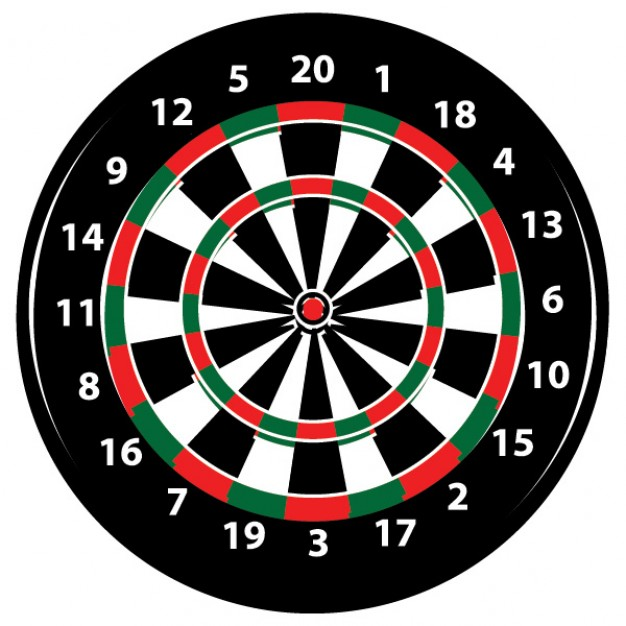
\includegraphics[width=0.5\textwidth]{darts}
\end{center}
\end{tcolorbox}
\paragraph{Вес} представленных гранат равен 0.5.
\paragraph{Дистанция} у гранат обычно Ближняя 5, Дальняя 20.
\paragraph{Центр Взрыва:} точка, из которой распространяется Взрыв.
\paragraph{Радиус Взрыва(РВ):} число метров, на которое распространяется Взрыв из центра Взрыва во все стороны. Если атака обладает свойством «Взрыв», то цель, против которой совершается проверка Доблести или Меткости, также считается находящейся в области Взрыва и получает Повреждения и прочие эффекты и от него тоже!
\paragraph{Сила Взрыва(СВ):} все существа, попавшие в радиус Взрыва, получают Пв, равные \textbf{|Сила Взрыва — БАЗщ — БДЗщ|}.
\paragraph{Газ:} газ распространяется в радиусе Взрыва и остается там какое-то время. Для определения длительности действия газа совершите проверку Неприятностей. Существа, вдохнувшие газ, страдают от эффектов яда, громко кашляют и чихают, если они еще в состоянии кашлять и чихать. Существа, имеющие Иммунитет к Ядовитым Пв, не подпадают под действие газа. В помещении увеличьте временные промежутки вдвое.
\trouble
{Штиль}%no sweat name
{Газ рассеивается чере 10 минут}%no sweat description
{Бриз}%tough day name
{Газ рассеивается через 5 минут}%tough day description
{Порыв ветра}%we have trouble name
{Газ рассеивается через 1 минуту}%we have trouble description
{Шторм}%fiasco name
{Газ рассеивается по истечении полного Круга}%fiasco description

\paragraph{Другие опасности Взрывов:} Взрывы опасны не только Повреждениями. Попавшие во Взрыв доспехи, щиты и прочие предметы, закрепленные на теле попавшего во Взрыв, получают \textbf{|Пв = Сила Взрыва — Прч|} и могут быть уничтожены. Если Взрыв достаточно силен, попавшие в него существа с воплями разлетаются в разные стороны! Если существо получает Повреждения от взрыва, его отбрасывает от центра Взрыва на \textbf{|Сила Взрыва — МСл отброшенного — МЛв отброшенного|} метров. Отброшенный получает столько Пв, сколько метров пролетел. Когда отброшенный сталкивается с другим существом, оно падает, если \textbf{|Сл отброшенного + БДЗщ отброшенного + БЩЗщ отброшенного $\pm$ БШР отброшенного| $\geq$ |Зщ существа + МСл существа $\pm$ Прч существа $\pm$ БШР существа|}. Существо получает 1 Пв за каждую единицу разницы не в свою пользу. В противном случае Пв получает отброшенный. Существо не может быть отброшено на большее число метров, чем получило Пв от Взрыва. Увеличьте расстояние броска в 2 раза за каждую категорию размера меньше Среднего и уменьшите в 2 раза за каждую категорию больше Среднего. Падения и столкновения наносят Дробящие Пв.
\newline
Если при подсчете дистанции отбрасывания получилось 0 или меньше, существо остается на месте.

\subsection{Спиок гранат}
\genAndGet{explosives}{explosives}
